\documentclass[../main.tex]{subfiles}
\begin{document}

The plan is to show all finitely generated reflection groups are in fact Coxeter groups, which admit a nice geometric classification. This follows\cite{Humphreys1990}

This is a rough outline of the structure:

\subsection{Reflection groups}

work in $n$-dimensional euclidean space $E$. This may be spoken about in the previous section?

The origin preserving reflections of $E$ are all contained in $O(E)$, this is also the smallest group containing all of these reflections.\citationneeded (easy induction i think?)
We also want to consider reflections that don't preserve the origin, or \textit{affine reflections} these will, similarly, all lie in the \textbf{affine orthogonal group} \[
AO(E) := E\rtimes O(E)
\] where $E$ acts on itself by translation.

A reflection in $E$ is an affine transformation $r\in AO(E)$ that  fixes some affine hyperplane $H$ (some translation of codimension $1$ subspace).

A group $W\leq AO(E)$ is a \textbf{reflection group} if it is generated by affine reflections. If we have $W\leq O(E)\leq AO(E)$ then we recover the definition used for reflection groups of regular polytopes discussed earlier.

From now on we will fix a reflection group $W$ and start referring to affine reflections as just reflections.

Let $\cH$ be the set of affine hyperplanes fixed by some reflection in $W$.

\begin{lemma}
    If $H\in\cH$ is an affine hyperplane and $s\in W$ is a reflection, $sH$ is also an affine hyperplane.
    \begin{proof}
        A hyperplane in any euclidean space is equivalently the locus\[
            \{v\in E \mid (v,\alpha)=0\}
        \] where $\alpha$ is the normal vector to the hyperplane. Thus an affine hyperplane with normal $\alpha$ and minimal distance from the origin $k$ will be \[
            \{v\in E \mid (v,\alpha)=k\}
        \] Now $sH$ will consists of points $sv$ such that $(v,\alpha)=k$, but as $s$ is $AO(E)$, it preserves the inner product so $(sv,s\alpha)=(v,\alpha)=k$ so\[
            sH = \{v\in E \mid (sv,s\alpha) = k\} = \{v\in E \mid (v,s^*s\alpha) = k\}
        \] where $s^*$ is the adjoint map.
    \end{proof}
\end{lemma}

Let $\Phi$ be the set of unit normal vectors to hyperplanes $H_i\in\cH$.

\begin{lemma}
    For all affine hyperplanes $H\in\cH$ with corresponding reflection $r\in W$, and reflections $s\in W$ the map $srs^{-1}$ is a reflection over the affine hyperplane $sH$.\begin{proof}
        
    \end{proof}
\end{lemma}

\begin{proposition}
    The action of $W$ on $E$ stabilises $\Phi$ and $\cH$.
    \begin{proof}
        Start by considering some affine hyperplane $H\in\cH$ with corresponding reflection $r\in W$, then for all $s\in W$ the map $srs^{-1}$ fixes $sH$ and has determinant $-1$ so is a reflection, therefore $sH\in\cH$ 
    \end{proof}
\end{proposition}

We can derive the Coxeter relations from $\Phi$, a group satisfying such relations is called Coxeter.

\begin{definition}
    We call a group $W$ \textbf{Coxeter} if it admits a presentation of the form:\[
    \abr{r_1,\ldots,r_n \mid (r_ir_j)^{m_{ij}}\text{ for all }i,j}
    \]
    where each $m_{ij}\in \bN\cup\{\infty\}$, and $m_{ii}=1$ for all $i$. For formal reasons, we will consider the pair $(W,R)$, where $R$ is the set of generators in the presentation, and call this a \textbf{Coxeter system}. We call a Coxeter system finite if $R$ is finite.
\end{definition}

\subsection{The fundamental domain}

The action of $W$ fixes $\Phi$ and $\cH$ so acts on the connexted componenets $E\setminus\cH$ called the set of \textbf{fundamental domains} for $W$. 

The reflections fixing hyperplanes bounding any single fundamental domain will generate $W$, such reflections (hyperplanes, roots) are called \textbf{simple}.

Show the action of $W$ on the fundamental domains is transitive

\subsection{Words}

The length of a word in terms of simple reflections corresponds to the number of plane between a fundamental domain and its image. This implies the action on fundamental domains is in fact \textbf{simply} transitive.

\begin{proposition}[Deletion condition]
    Given an unreduced expression $w=r_1\cdots r_k$ there exists $1\leq i < j \leq k$ such that $w=r_1\cdots\hat{r_i}\cdots\hat{r_j}\cdots r_k$, where the hat means ommitance.
\end{proposition}

\begin{proposition}[Exchange condition]
    For $w=r_1\cdots r_k$ a not necessarily reduced expression and some simple $r\in W$ with $l(wr)<l(w)$, then there exists an $1\leq i\leq k$ s.t. $wr = r_1\cdots\hat{r_i}\cdots r_k$.
\end{proposition}

\begin{theorem}
    Any non-trivial relation in a reflection group is a consequence of the Coxeter relations.
\end{theorem}

\subsection{Classification}

To any finite Coxeter system $(W,R)$ we can associate an undirected graph called its \textbf{Coxeter diagram} by the following rules:\begin{itemize}
    \item Draw a node $i$ for each $r_i\in R$;
    \item For each relation $(r_i r_j)^{m_{ij}}$ with $m_{ij}>2$ draw an edge between $i$ and $j$ and label it with $m_{ij}$.
\end{itemize}

This process can be reversed to obtain a Coxeter system from any Coxeter diagram. This correspondence will associate the graph:
\begin{figure}[!h]
\centering
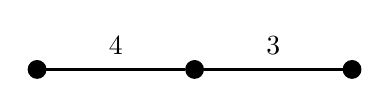
\begin{tikzpicture}
    \begin{scope}[every node/.style={circle, fill=black, draw, thick, minimum size = 6pt, inner sep=0pt}]
        \node (1) at (0,0) {};
        \node (2) at (2,0) {};
        \node (3) at (4,0) {};
    \end{scope}

    \begin{scope}[every edge/.style={draw,very thick}]
        \path [-] (1) edge (2);
        \path [-] (2) edge (3);
        \node at (1,0.3) {$4$};
        \node at (3,0.3) {$3$};
    \end{scope}
\end{tikzpicture}
\end{figure}

to the group presentation: \[
\abr{r_1,r_2,r_3 \ \middle| \ r_1^2 = r_2^2 = r_3^2 = e, \ (r_1r_2)^4 = (r_2r_3)^3 = (r_1r_3)^2 = e}
\]

For brevity the $3$ labels will often  be excluded.

\begin{itemize}
    \item show the graph is well defined up isometryish
    \item disjoint unions of graphs correspond to products of groups
    \item bilinear form of a coxeter group
    \item if positive definite, the coxeter group is finite
    \item classify positive-definite forms
    \item all of which can be seen as reflection groups of regular polyhedra. some of which will be described in the previous section?
\end{itemize}

\begin{figure}[H]
\resizebox{\textwidth}{!}{
\begin{tikzpicture}
    \begin{scope}[shift={(0,0)}]
        \node at (0,0) {$A_n$};
        \begin{scope}[every node/.style={circle, fill=black, draw, thick, minimum size = 6pt, inner sep=0pt}]
            \node (1) at (2,0) {};
            \node (2) at (4,0) {};
            \node (3) at (6,0) {};
            \node (n-2) at (10,0) {};
            \node (n-1) at (12,0) {};
            \node (n) at (14,0) {};
        \end{scope}
        \node (3a) at (7,0) {};
        \node (3b) at (9,0) {};
        \begin{scope}[every edge/.style={draw,very thick}]
            \path [-] (1) edge (2);
            \path [-] (2) edge (3a);
            \path [loosely dashed] (3a.west) edge (3b.east);
            \path [-] (3b) edge (n-1);
            \path [-] (n-1) edge (n);
        \end{scope}
        \node at (16,0) {$(n\geq 1)$};
    \end{scope}

    \begin{scope}[shift={(0,-1.5)}]
        \node at (0,0) {$BC_n$};
        \begin{scope}[every node/.style={circle, fill=black, draw, thick, minimum size = 6pt, inner sep=0pt}]
            \node (1) at (2,0) {};
            \node (2) at (4,0) {};
            \node (3) at (6,0) {};
            \node (n-2) at (10,0) {};
            \node (n-1) at (12,0) {};
            \node (n) at (14,0) {};
        \end{scope}
        \node (3a) at (7,0) {};
        \node (3b) at (9,0) {};
        \begin{scope}[every edge/.style={draw,very thick}]
            \path [-] (1) edge (2);
            \path [-] (2) edge (3a);
            \path [loosely dashed] (3a.west) edge (3b.east);
            \path [-] (3b) edge (n-1);
            \path [-] (n-1) edge (n);
            \node at (13,0.3) {$4$};
        \end{scope}
        \node at (16,0) {$(n\geq 2)$};
    \end{scope}

    \begin{scope}[shift={(0,-5)}]
        \node at (0,0) {$D_n$};
        \begin{scope}[every node/.style={circle, fill=black, draw, thick, minimum size = 6pt, inner sep=0pt}]
            \node (1) at (2,0) {};
            \node (2) at (4,0) {};
            \node (3) at (6,0) {};
            \node (n-2) at (10,0) {};
            \node (n-1) at (12,0) {};
            \node (n-1a) at (12,2) {};
            \node (n) at (14,0) {};
        \end{scope}
        \node (3a) at (7,0) {};
        \node (3b) at (9,0) {};
        \begin{scope}[every edge/.style={draw,very thick}]
            \path [-] (1) edge (2);
            \path [-] (2) edge (3a);
            \path [loosely dashed] (3a.west) edge (3b.east);
            \path [-] (3b) edge (n-1);
            \path [-] (n-1) edge (n-1a);
            \path [-] (n-1) edge (n);
        \end{scope}
        \node at (16,0) {$(n\geq 4)$};
    \end{scope}

    \begin{scope}[shift={(0,-8.5)}]
        \node at (0,0) {$E_6$};
        \begin{scope}[every node/.style={circle, fill=black, draw, thick, minimum size = 6pt, inner sep=0pt}]
            \node (1) at (2,0) {};
            \node (2) at (4,0) {};
            \node (3) at (6,0) {};
            \node (4) at (6,2) {};
            \node (5) at (8,0) {};
            \node (6) at (10,0) {};
        \end{scope}
        \begin{scope}[every edge/.style={draw,very thick}]
            \path [-] (1) edge (2);
            \path [-] (2) edge (3);
            \path [-] (3) edge (4);
            \path [-] (3) edge (5);
            \path [-] (5) edge (6);
        \end{scope}
    \end{scope}

    \begin{scope}[shift={(0,-12)}]
        \node at (0,0) {$E_7$};
        \begin{scope}[every node/.style={circle, fill=black, draw, thick, minimum size = 6pt, inner sep=0pt}]
            \node (1) at (2,0) {};
            \node (2) at (4,0) {};
            \node (3) at (6,0) {};
            \node (4) at (8,0) {};
            \node (5) at (8,2) {};
            \node (6) at (10,0) {};
            \node (7) at (12,0) {};
        \end{scope}
        \begin{scope}[every edge/.style={draw,very thick}]
            \path [-] (1) edge (2);
            \path [-] (2) edge (3);
            \path [-] (3) edge (4);
            \path [-] (4) edge (5);
            \path [-] (4) edge (6);
            \path [-] (6) edge (7);
        \end{scope}
    \end{scope}

    \begin{scope}[shift={(0,-15.5)}]
        \node at (0,0) {$E_8$};
        \begin{scope}[every node/.style={circle, fill=black, draw, thick, minimum size = 6pt, inner sep=0pt}]
            \node (1) at (2,0) {};
            \node (2) at (4,0) {};
            \node (3) at (6,0) {};
            \node (4) at (8,0) {};
            \node (5) at (10,0) {};
            \node (6) at (10,2) {};
            \node (7) at (12,0) {};
            \node (8) at (14,0) {};
        \end{scope}
        \begin{scope}[every edge/.style={draw,very thick}]
            \path [-] (1) edge (2);
            \path [-] (2) edge (3);
            \path [-] (3) edge (4);
            \path [-] (4) edge (5);
            \path [-] (5) edge (6);
            \path [-] (5) edge (7);
            \path [-] (7) edge (8);
        \end{scope}
    \end{scope}

    \begin{scope}[shift={(0,-17)}]
        \node at (0,0) {$F_4$};
        \begin{scope}[every node/.style={circle, fill=black, draw, thick, minimum size = 6pt, inner sep=0pt}]
            \node (1) at (2,0) {};
            \node (2) at (4,0) {};
            \node (3) at (6,0) {};
            \node (4) at (8,0) {};
        \end{scope}
        \begin{scope}[every edge/.style={draw,very thick}]
            \path [-] (1) edge (2);
            \path [-] (2) edge (3);
            \path [-] (3) edge (4);
            \node at (5,0.3) {$4$};
        \end{scope}
    \end{scope}

    \begin{scope}[shift={(0,-18.5)}]
        \node at (0,0) {$H_3$};
        \begin{scope}[every node/.style={circle, fill=black, draw, thick, minimum size = 6pt, inner sep=0pt}]
            \node (1) at (2,0) {};
            \node (2) at (4,0) {};
            \node (3) at (6,0) {};
        \end{scope}
        \begin{scope}[every edge/.style={draw,very thick}]
            \path [-] (1) edge (2);
            \path [-] (2) edge (3);
            \node at (3,0.3) {$5$};
        \end{scope}
    \end{scope}

    \begin{scope}[shift={(0,-20)}]
        \node at (0,0) {$H_4$};
        \begin{scope}[every node/.style={circle, fill=black, draw, thick, minimum size = 6pt, inner sep=0pt}]
            \node (1) at (2,0) {};
            \node (2) at (4,0) {};
            \node (3) at (6,0) {};
            \node (4) at (8,0) {};
        \end{scope}
        \begin{scope}[every edge/.style={draw,very thick}]
            \path [-] (1) edge (2);
            \path [-] (2) edge (3);
            \path [-] (3) edge (4);
            \node at (3,0.3) {$5$};
        \end{scope}
    \end{scope}

    \begin{scope}[shift={(0,-21.5)}]
        \node at (0,0) {$I_2(m)$};
        \begin{scope}[every node/.style={circle, fill=black, draw, thick, minimum size = 6pt, inner sep=0pt}]
            \node (1) at (2,0) {};
            \node (2) at (4,0) {};
        \end{scope}
        \begin{scope}[every edge/.style={draw,very thick}]
            \path [-] (1) edge (2);
            \node at (3,0.3) {$m$};
            \node at (6,0) {$(m\geq 4)$};
        \end{scope}
    \end{scope}
\end{tikzpicture}
}
\end{figure}

\end{document}